\documentclass[10pt,border=2mm]{standalone}
\usepackage[T1]{fontenc}
\usepackage{times}
\usepackage{amsmath}
\usepackage{xcolor}
\usepackage{tikz}
\usetikzlibrary{arrows.meta,positioning,fit,backgrounds,calc}
\newcommand{\Ktool}{$K_{\text{tool}}$}
\newcommand{\Kdisc}{$K_{\text{disc}}$}
\definecolor{cFedot}{HTML}{009E73}
\definecolor{cAuto}{HTML}{0072B2}
\definecolor{cTerm}{HTML}{D55E00}
\definecolor{cLayer}{HTML}{F0E442}
\definecolor{ink}{HTML}{1A1A1A}
\definecolor{muted}{HTML}{6E6E6E}
\definecolor{ctx}{HTML}{9A9A9A}
\begin{document}
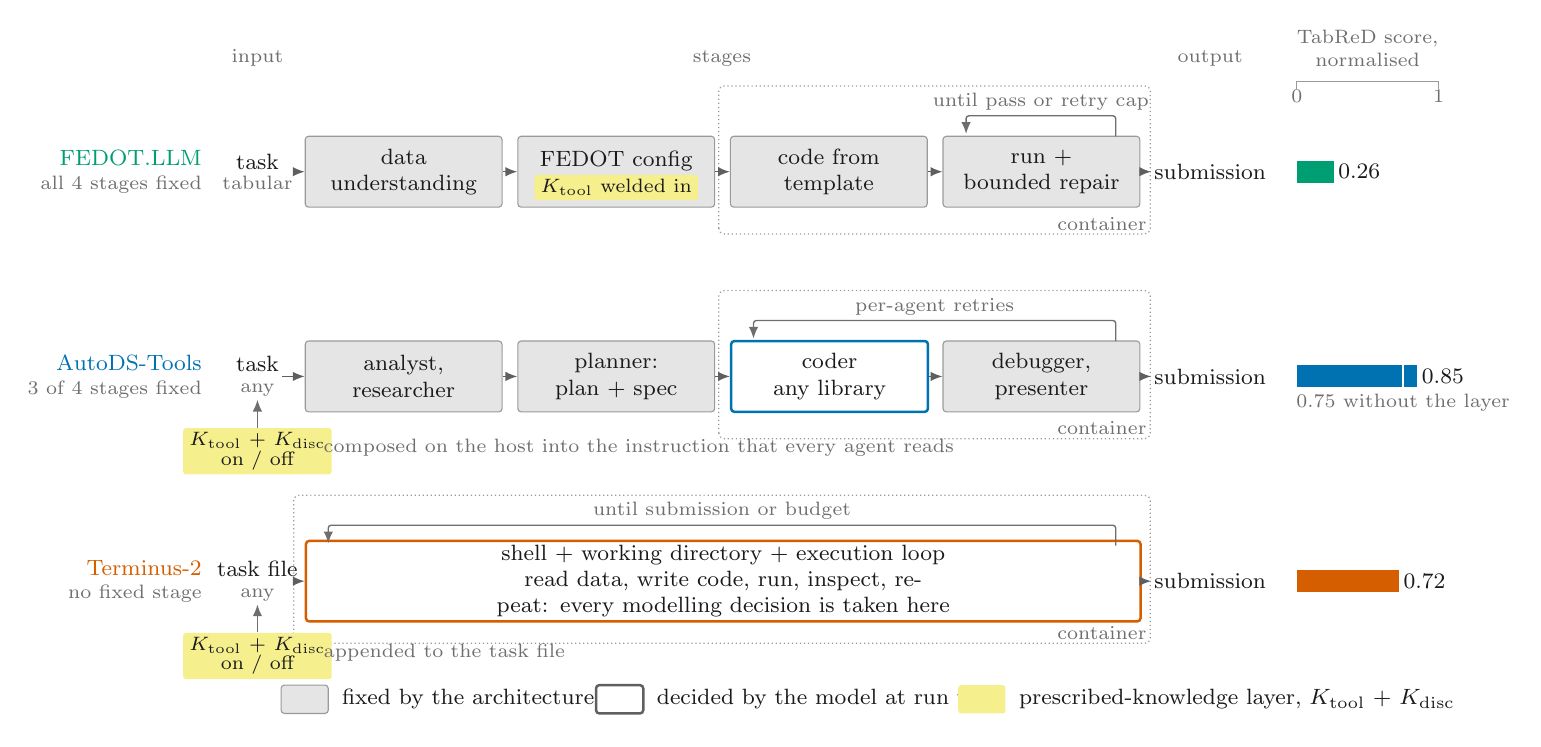
\begin{tikzpicture}[x=1mm,y=1mm, font=\footnotesize, text=ink,
  stage/.style = {draw=ctx, fill=black!10, rounded corners=1.2pt, line width=0.4pt,
                  minimum height=9mm, minimum width=25mm, text width=23.5mm,
                  align=center, inner xsep=0.5pt, inner ysep=1.5pt},
  free/.style  = {stage, fill=white, line width=0.9pt},
  chip/.style  = {fill=cLayer!60, rounded corners=1pt, inner xsep=2.2pt, inner ysep=1.6pt,
                  font=\scriptsize, align=center},
  io/.style    = {inner sep=1pt, align=center},
  arr/.style   = {-{Latex[length=1.5mm,width=1.2mm]}, draw=ink!70, line width=0.5pt},
  loop/.style  = {arr, draw=muted, rounded corners=1pt},
  env/.style   = {rounded corners=2pt, draw=ctx, densely dotted, line width=0.45pt},
  lbl/.style   = {font=\scriptsize, text=muted, inner sep=1pt, align=center},
  lane/.style  = {anchor=east, align=right, inner sep=0pt},
]
% ---- geometry --------------------------------------------------------------
\def\xLane{21}     % right edge of lane labels
\def\xTask{28}     % centre of the input node
\def\xA{34}\def\xB{61}\def\xC{88}\def\xD{115}   % left edges of the 4 stage columns
\def\wS{25}        % stage width
\def\xOut{149}     % centre of the output node
\def\xBar{160}     % score bar origin
\def\wBar{18}      % score bar span for score = 1
\def\yA{0}\def\yB{-26}\def\yC{-52}
\def\hRow{9}

% ---- header ----------------------------------------------------------------
\node[lbl, anchor=south] at (\xTask,13) {input};
\node[lbl, anchor=south] at ({(\xA+\xD+\wS)/2},13) {stages};
\node[lbl, anchor=south] at (\xOut,13) {output};
\node[lbl, anchor=south, text width=26mm] at ({\xBar+\wBar/2},13) {TabReD score,\\normalised};
\draw[ctx, line width=0.4pt] (\xBar,11.5) -- ++(\wBar,0);
\foreach \t/\l in {0/0, 1/1} \draw[ctx, line width=0.4pt] ({\xBar+\t*\wBar},11.5) -- ++(0,-1)
   node[lbl, below, inner sep=0.3pt] {\l};

% ---- helpers ---------------------------------------------------------------
% loop above the span [#1,#2] in row #3, label #4
\newcommand{\iterloop}[4]{%
  \draw[loop] ({#2-3},{#3+\hRow/2}) -- ({#2-3},{#3+\hRow/2+2.6}) -- ({#1+3},{#3+\hRow/2+2.6}) -- ({#1+3},{#3+\hRow/2+0.3});
  \node[lbl, anchor=south] at ({(#1+#2)/2},{#3+\hRow/2+2.9}) {#4};}
% dotted container frame around the span [#1,#2] in row #3, named #4
\newcommand{\envframe}[4]{%
  \begin{scope}[on background layer]
    \draw[env] ({#1-1.4},{#3-\hRow/2-3.4}) rectangle ({#2+1.4},{#3+\hRow/2+6.4});
  \end{scope}
  \node[lbl, anchor=south east, inner sep=1.2pt] at ({#2+1.4},{#3-\hRow/2-3.4}) {container};}
% score bar in row #1, value #2, colour #3, label #4
\newcommand{\scorebar}[4]{%
  \fill[#3] (\xBar,{#1-1.4}) rectangle ({\xBar+#2*\wBar},{#1+1.4});
  \node[anchor=west, inner sep=1.5pt] at ({\xBar+#2*\wBar},#1) {#4};}

% ============================ row 1: FEDOT.LLM ==============================
\node[lane, text=cFedot] at (\xLane,\yA) {FEDOT.LLM\\[-1pt]{\scriptsize\color{muted}all 4 stages fixed}};
\node[io] (t1) at (\xTask,\yA) {task\\[-2pt]{\scriptsize\color{muted}tabular}};
\node[stage, anchor=west] (a1) at (\xA,\yA) {data\\understanding};
\node[stage, anchor=west] (b1) at (\xB,\yA) {FEDOT config\\\phantom{x}};
\node[chip, anchor=south] at ([yshift=0.9mm]b1.south) {\Ktool{} welded in};
\node[stage, anchor=west] (c1) at (\xC,\yA) {code from\\template};
\node[stage, anchor=west] (d1) at (\xD,\yA) {run $+$\\bounded repair};
\node[io] (e1) at (\xOut,\yA) {submission};
\foreach \i/\j in {t1/a1,a1/b1,b1/c1,c1/d1,d1/e1} \draw[arr] (\i) -- (\j);
\iterloop{\xD}{\xD+\wS}{\yA}{until pass or retry cap}
\envframe{\xC}{\xD+\wS}{\yA}{env1}
\scorebar{\yA}{0.26}{cFedot}{0.26}

% ============================ row 2: AutoDS-Tools ============================
\node[lane, text=cAuto] at (\xLane,\yB) {AutoDS-Tools\\[-1pt]{\scriptsize\color{muted}3 of 4 stages fixed}};
\node[io] (t2) at (\xTask,\yB) {task\\[-2pt]{\scriptsize\color{muted}any}};
\node[stage, anchor=west] (a2) at (\xA,\yB) {analyst,\\researcher};
\node[stage, anchor=west] (b2) at (\xB,\yB) {planner:\\plan $+$ spec};
\node[free, draw=cAuto, anchor=west] (c2) at (\xC,\yB) {coder\\any library};
\node[stage, anchor=west] (d2) at (\xD,\yB) {debugger,\\presenter};
\node[io] (e2) at (\xOut,\yB) {submission};
\foreach \i/\j in {t2/a2,a2/b2,b2/c2,c2/d2,d2/e2} \draw[arr] (\i) -- (\j);
\iterloop{\xC}{\xD+\wS}{\yB}{per-agent retries}
\envframe{\xC}{\xD+\wS}{\yB}{env2}
\node[chip, anchor=north] (k2) at (\xTask,{\yB-6.5}) {\Ktool{} $+$ \Kdisc\\[-1pt]on / off};
\draw[arr, draw=muted] (k2.north) -- (t2.south);
\node[lbl, anchor=west, align=left] at ({\xA+2},{\yB-9.1}) {composed on the host into the instruction that every agent reads};
\scorebar{\yB}{0.85}{cAuto}{0.85}
\draw[white, line width=0.6pt] ({\xBar+0.75*\wBar},{\yB-1.4}) -- ++(0,2.8);
\node[lbl, anchor=north] at ({\xBar+0.75*\wBar},{\yB-1.8}) {0.75 without the layer};

% ============================ row 3: Terminus-2 ==============================
\node[lane, text=cTerm] at (\xLane,\yC) {Terminus-2\\[-1pt]{\scriptsize\color{muted}no fixed stage}};
\node[io] (t3) at (\xTask,\yC) {task file\\[-2pt]{\scriptsize\color{muted}any}};
\node[free, draw=cTerm, anchor=west, minimum width={(\xD+\wS-\xA)*1mm}, text width={(\xD+\wS-\xA-3)*1mm}] (a3) at (\xA,\yC)
     {shell $+$ working directory $+$ execution loop\\read data, write code, run, inspect, repeat: every modelling decision is taken here};
\node[io] (e3) at (\xOut,\yC) {submission};
\draw[arr] (t3) -- (a3); \draw[arr] (a3) -- (e3);
\iterloop{\xA}{\xD+\wS}{\yC}{until submission or budget}
\envframe{\xA}{\xD+\wS}{\yC}{env3}
\node[chip, anchor=north] (k3) at (\xTask,{\yC-6.5}) {\Ktool{} $+$ \Kdisc\\[-1pt]on / off};
\draw[arr, draw=muted] (k3.north) -- (t3.south);
\node[lbl, anchor=west, align=left] at ({\xA+2},{\yC-9.1}) {appended to the task file};
\scorebar{\yC}{0.72}{cTerm}{0.72}

% ---- legend ------------------------------------------------------------------
\begin{scope}[shift={(\xA,-67)}]
  \node[stage, minimum width=6mm, minimum height=3.6mm, text width=5mm] at (0,0) {};
  \node[anchor=west] at (3.5,0) {fixed by the architecture};
  \node[free, draw=ink!70, minimum width=6mm, minimum height=3.6mm, text width=5mm] at (40,0) {};
  \node[anchor=west] at (43.5,0) {decided by the model at run time};
  \node[chip, minimum width=6mm, minimum height=3.6mm] at (86,0) {};
  \node[anchor=west] at (89.5,0) {prescribed-knowledge layer, \Ktool{} $+$ \Kdisc};
\end{scope}
\end{tikzpicture}
\end{document}
